\section{Архитектура и модули системы}

Разработанное программное средство состоит из следующих модулей:
\begin{itemize}
    \item модуль выделения признаков почерка;
    \item модуль определения параметров личности;
    \item модуль контроля доступа;
    \item модуль доступа к базе данных.
\end{itemize}

Вышеописанные модули опираются на следующие группы классов, разработанные в рамках дипломного проекта:
\begin{itemize}
    \item Набор классов для сегментации изображения на строки, слова, символы и выделения признаков. Написан на языке Scala с использование сторонней00 библиотеки OpenCV.
    \item Набор классов машинного обучения (для классификации признаков текста). Написан на языке программирования Scala и содержит реализацию алгоритма основанного на методе опорных векторов (Support Vector Machine), о котором будет рассказано далее.
    \item Набор классов для контроля доступа. Написана на языке Scala. Содержит классы для регистрации, авторицации и управлением сессией пользователя. Основан на стандарте JSON Web Token (JWT).
    \item Набор классов для организации храниения и доступа в авторизационным данным пользователя и коллекции обработанных изображений.
\end{itemize}

Далее будет подробно описана структура и назначения каждого модуля.

\afterpage{
  \begin{landscape}
  \thispagestyle{lscape}
  \begin{figure}[t!]
  \centering
    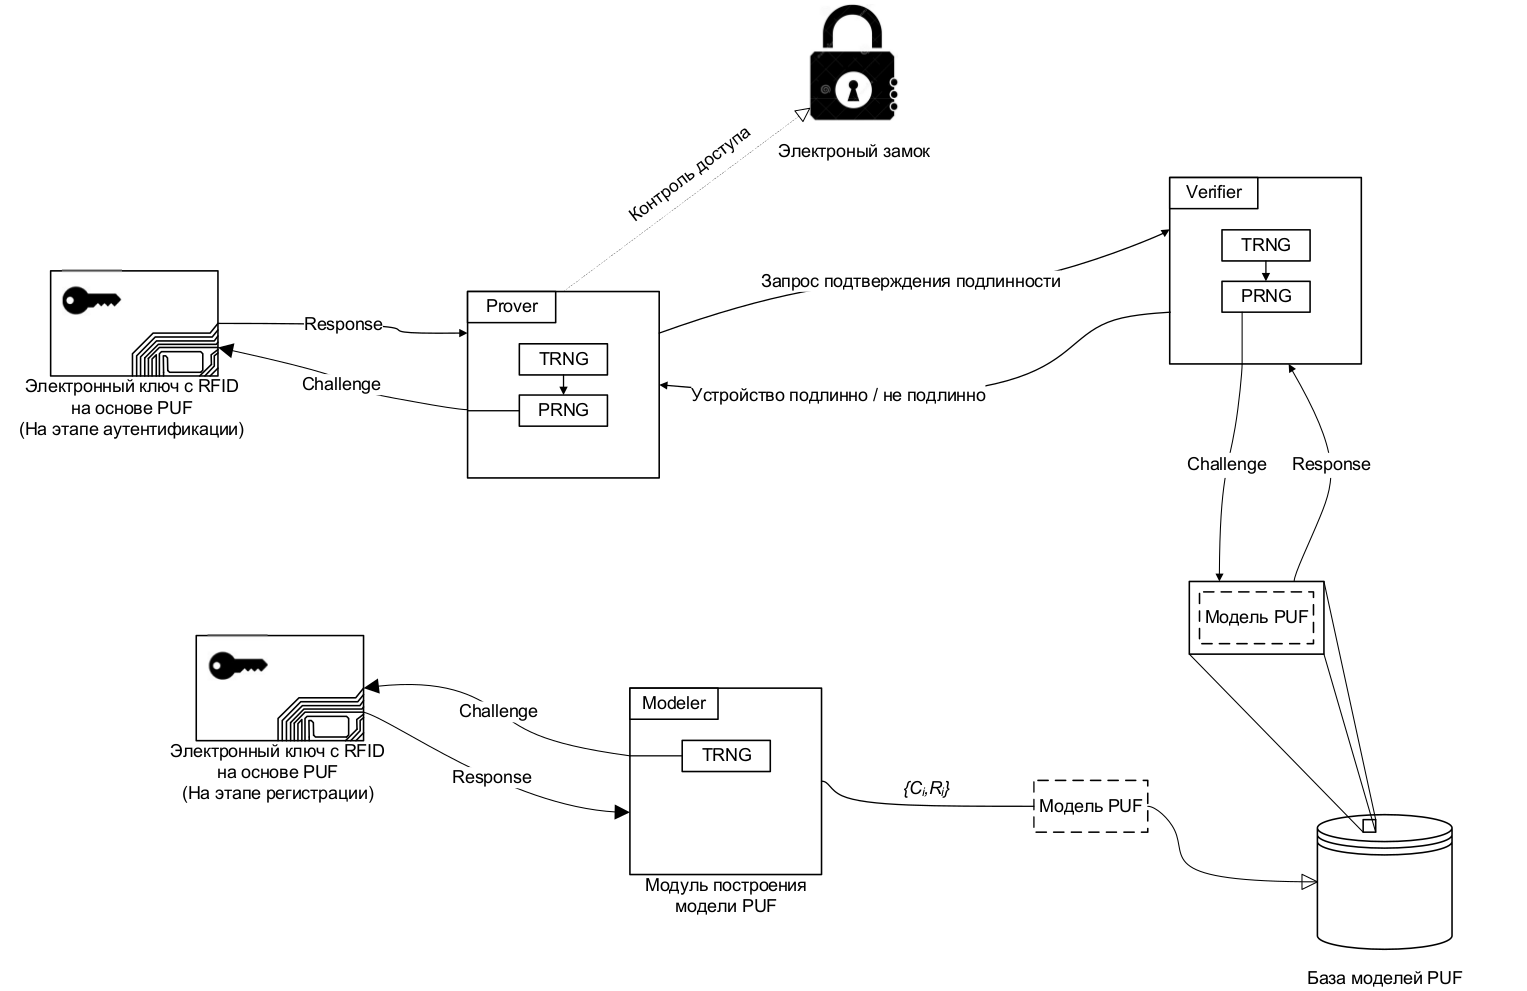
\includegraphics[scale=0.40]{figures/flow.png}
    \caption{ Схема работы программной системы }
    \label{fig:architecture:flow}
  \end{figure}
  \end{landscape}
}

\subsection{Модуль определения параметров личности}

Для определения параметров личности по признаком рукописного текста был выбран классификатор на основе метода опорных векторов -- широко используемый метод машинного обучения~\cite{manning_ir}, который при своей относительной простоте реализации, позволяет добиться очень неплохих результатов классификации.

Метод опорных векторов (\emph{SVM, support vector machine}) – семейство схожих алгоритмов обучения с учителем, использующихся для задач классификации и регрессионного анализа. Особым свойством метода опорных векторов является непрерывное уменьшение эмпирической ошибки классификации и увеличение зазора, поэтому метод также известен как метод классификатора с максимальным зазором.~\cite{mitchell_ml, wiki_SVM}:

Параметры текста представляют собой непрерывные величины подчиняющиеся нормальному распределению, исходя из этого в качестве ядер используются радиально-базисная функция Гаусса~\cite{gauss_wiki}.

\begin{equation}
  \label{eq:architecture:gaussian_core}
  k(x, x^{'}) = \exp(-\frac{\left|\left| x - x^{'} \right|\right|}{2\sigma_{}^2})
\end{equation}
\begin{explanation}
где & $x^{'}$ & среднее значение параметра, рассчитанное для объектов, принадлежащих
классу $C$; \\
    & $ \sigma_{}^2 $ & дисперсия значания параметра объектов из класс $C$.
\end{explanation}

Дисперсия значения параметра:
\begin{equation}
  \label{eq:architecture:dispersion}
  \sigma_{}^2 = \frac{1}{n - 1} \sum\limits_{x \in C} (x_i - \overline{x_{}}^2)
\end{equation}

\begin{figure}[!h]
    \centering
    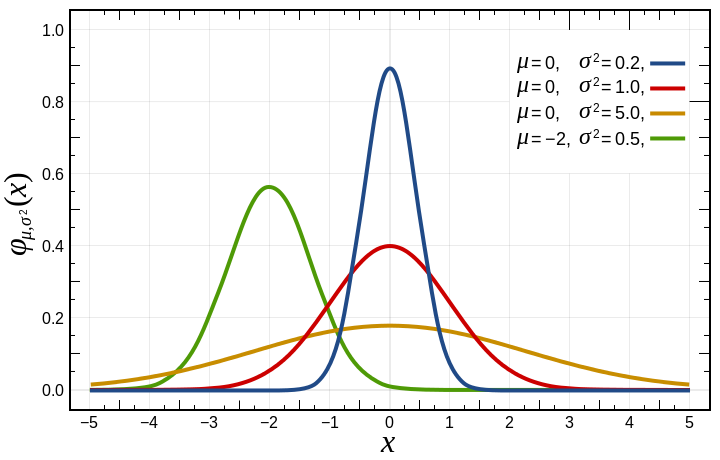
\includegraphics[width=0.85\textwidth]{figures/gauss.png}
    \caption{График функции плотности вероятности для нормального распределения}
    \label{fig:architecture:normal_pd}
\end{figure}

\subsection{Модуль выделения признаков почерка}
Основным функциями данного модуля является:
\begin{itemize}
  \item подготовка изображения к обработке (бинаризация, удаление шумов);
  \item сегментация текста (строки, слова, символы);
  \item выделения признаков подчерка.
\end{itemize}

На это этапе обработки используется алгоритм линейной бинаризации по пороговому значению доминантного цвета, посколько обработке подверкается образцы почерка с высокой вероятностью это будет цвет чернил.
Математическое выражение линейной бинаризации выглядит следующим образов:

\begin{equation}
  \label{eq:architecture:liner_binarisation}
 \left \{
  \begin{tabular}{l}
   x <  T, x = 0 \\
   x $ \geq $ T, x = 255
  \end{tabular}
   \right .
\end{equation}
\begin{explanation}
где & $ x $ & значения яркости цвета пикселя; \\
    & Т & порог бинаризации.
\end{explanation}

Для удаления шумов используется фильтр максимума - минимума. Алгоритм работы данного фильтра основан на замене текущего пикселя на пиксель с максимальной яркостью из его окресности при первом проходе и на пиксель с минимальной при повторном. Данный алгоритм хорошо справляется с импульсными шумами и шумами типа <<соль и перец>>.

Следующий этапам является сегментация изображения, а первой стадией сегментации является сегментация строк. 
Задача выделения строк сводиться к нахождению верхних и нижних граней строк текста на исходном изображении. Алгоритм сегментации строк основывается на том, что средняя яркость в изображениях межстрочных промежутках существенно ниже средней яркости в изображениях текстовых строк~\cite{cv_text_image_segmentator}.

Первым этапом необходимо для всех пиксельных строк исходного изображения находим их средние значения яркости
\begin{displaymath}s_j = s_j(B) = \frac{1}{n}\cdot\sum\limits_{i=1}^{n} b_{ij}\end{displaymath}

Затем определяем среднее значение яркости всего изображения
\begin{displaymath}s(B) = \frac{1}{m}\cdot\sum\limits_{j=1}^{m} s_j(B)\end{displaymath}

Средняя яркость в межстрочных промежутках текста должна быть невелика (в идеальном случае она равна нулю). Поэтому яркость верхней границы текстовой строки можно выразить через среднюю яркость изображения
\begin{displaymath}s^{t} = k^{t} * s(B)\end{displaymath}

где 0<kt<1 - коэффициент

Аналогично яркость нижней границы текстовой строки, также может быть выражена через среднюю яркость всего изображения
sb= kb * s(B)

где 0<kb<1 - коэффициент

Работа алгоритма сегментации строк заключается в последовательном просмотре массива средних значений (s1,...,sm) и выявлении множества пар индексов (sti,sbi) пиксельных строк, соответствующих верхней sti и нижней sbi граням изображения строки номер i, удовлетворяющих следующим условиям.

Условия верхней границы текстовой строки:
\begin{itemize}
  \item яркость текущей пиксельной строки превышает границу $ s^{t} $
  \item яркость двух предыдущих пиксельных строк ниже этой границы
  \item яркость трех последующих строк выше границы $ s^{b} $
\end{itemize}

Следовательно должно выполняться логическое условие:
\begin{displaymath}(s_{i-2} < s^{t}) \wedge (s_{i-1} < s^{t}) \wedge (s_i > s^{b}) \wedge (s_{i+1} > s^{b}) \wedge (s_{i+2} > s^{b}) \wedge (s_{i+3} > s^{b})\end{displaymath}

Условия нижней границы текстовой строки.
\begin{itemize}     
  \item было зафиксировано начало области
  \item яркость текущей пиксельной строки превышает границу $ s^{t} $
  \item яркость последующей пиксельной строки ниже границы $ s^{b} $
\end{itemize}
     
или

\begin{itemize}
   \item было зафиксировано начало области
   \item яркость трех последующих строк ниже границы $ s^{b} $
\end{itemize}

Следовательно должно выполняться логическое условие:
\begin{displaymath}((s_{i+1} < s^{b}) \wedge (s_{i+2} < s^{b}) \wedge (s_{i+3} < s^{b}) \vee ((s_i > s^{t}) \wedge (s_{i+1} < s^{b})))\end{displaymath}

В результате формируется множество пар индексов верхних и нижних граней строк. Разность между этими индексами дает высоты текстовых строк. Однако такой алгоритм находит среднюю высоту каждой текстовой строки и "срезает" символы, выступающие по высоте за эту среднюю высоту.

Чтобы избежать этого, необходимо расширить найденные границы. Можно предложить следующий алгоритм расширения границ. Среди найденных текстовых строк определяется строка с минимальной высотой Hmin и, затем все границы с каждой стороны расширяются на величину 0.3 * Hmin. Это не приводит к слиянию строк, т.к. межстрочные интервалы текста, как правило, больше чем высота строки.

Таким образом, в результате работы алгоритма на исходном изображении отмечается положение всех текстовых строк.  

Алгоритмы сегментации слов и символом сходи с алгоритмом сегментации строк. Основными отличиями являются необходимость построения карты яркости столбцов, а не строк, а так наличие дополнительных этапов обработки. Такими этапоми являются приминение <<размазывающего>> фильтра при сегментации слов и удаление ложных границ после сегментации символов. 

Следующей функцией данного модуля является выделение из изображения признаков текста:
\begin{itemize}
  \item наклон символов;
  \item наклон строк;
  \item интервал между символами;
  \item интервал между строками;
  \item частота текста;
  \item сила нажима.
\end{itemize}

\subsection{Слой взаимодействия с устройствами}
Данная часть программного средства представляет собой абстракцию над любыми типами устройств с PUF (как аппаратными, так и программно симулированными) и предоставляет единый интерфейс взаимодействия с ними. Таким образом, благодаря этому слою, все части программного средства могут единообразно обращаться к любому подключённому устройству с целью регистрации или аутентификации вне зависимости от реализации этого устройства. Для эффективного взаимодействия в рамках этих целей достаточно лишь иметь доступ к собственно функции PUF для обмена сигналами и к некоторым её свойствам, в частности -- ожидаемой длине входного сигнала. С точки зрения программного кода этот слой реализован в виде абстрактного класса device.Device, исходный код которого представлен в листинге \ref{lst:architecture:device}.

\lstinputlisting[
    style=commonstyle,
    caption={Слой взаимодействия с устройствами, класс Device},
    label=lst:architecture:device
]{src/device.py}

В текущей поставке программной системы реализован класс SoftwareArbiter, который представляет собой обертку над программно-симулированным устройством с PUF типа арбитр. Объект класса SoftwareArbiter инициализируется заранее рассчитанными значениями задержек на узлах PUF. Для использования SoftwareArbiter, как и любого другого класса, реализующего методы Device, достаточно вызвать метод объекта SoftwareArbiter.f с битовым массивом значений управляющих сигналов в качестве аргумента. Применительно к PUF типа арбитр функция f рассчитывает выходной бит по следующей формуле:

\begin{equation}
  \label{eq:architecture:arbiter}
  \sum_{j=1}^{N}(-1)^{\rho_j}\delta_j + \delta_{N+1}\mathop{\lessgtr}_{r=1}^{r=0} 0\text{\,,}
\end{equation}
\begin{explanation}
где & $ \rho_j $ & количество единичных битов входного сигнала; \\
    & $ N $ & количество звеньев в цепи; \\
    & $ \delta_j $ & значение задержки на каждом звене. \\
\end{explanation}



\subsection{Библиотека протокола аутентификации}
Реализация протокола аутентификации, используемая в разработанном ПО, является частным случаем т.н. протоколов аутентификации на основе поиска подстроки (substring matching-based authentication protocol). Данный тип протоколов представил в 2012 году M. Majzoobi под названием \emph{Slender  PUF  protocol}~\cite{slender_puf}.

Протокол предназначен для использования со стойкими физически неклонируемыми функциями (Strong PUFs), является очень легковесным и отлично подходит для реализации в устройствах и системах с ограниченными вычислительными ресурсами. В отличие от уже устоявшейся парадигмы, данный протокол не подразумевает раскрытие полной последовательности выходных сигналов, даже в зашифрованном или трансформированном каким-либо другим способом виде. Вместо этого, из последовательности выделяются случайные части и отсылаются как доказательство подлинности. Для аутентификации устройства проверяющая сторона использует заранее сгенерированные шаблоны выходной последовательности (response patterns).

При корректной реализации протокол может обеспечить превосходную устойчивость против любых известных атак, использующих построение модели PUF-устройства с помошью методов машинного обучения. В дополнение к этому, в протокол сразу заложена коррекция ошибок, которые могут возникнуть при получении выходной строки по уже рассмотренным причинам. Благодаря этому, не требуется реализация сторонних алгоритмов коррекции ошибок, отнимающих драгоценные ресурсы, как не требуется и реализация хэш-функций, нечетких экстракторов (fuzzy extractors), предложенных в ранее известных протоколах аутентификации на основе ФНФ.

В основе протокола лежит построение компактной модели PUF методом машинного обучения. При этом оговаривается, что обучение модели должно быть доступно только на этапе регистрации, после чего возможность извлечения полных выходных последовательностей должна быть заблокировано физическим путем.

Библиотека протокола аутентификации представляет собой небольшой набор классов и функций, реализующих протокол аутентификации PUF на основе поиска подстроки. Сама схема протокола аутентификации продемонстрирована на рисунке \ref{fig:architecture:protocol}.

% \afterpage{
\begin{figure}[!h]
    \centering
    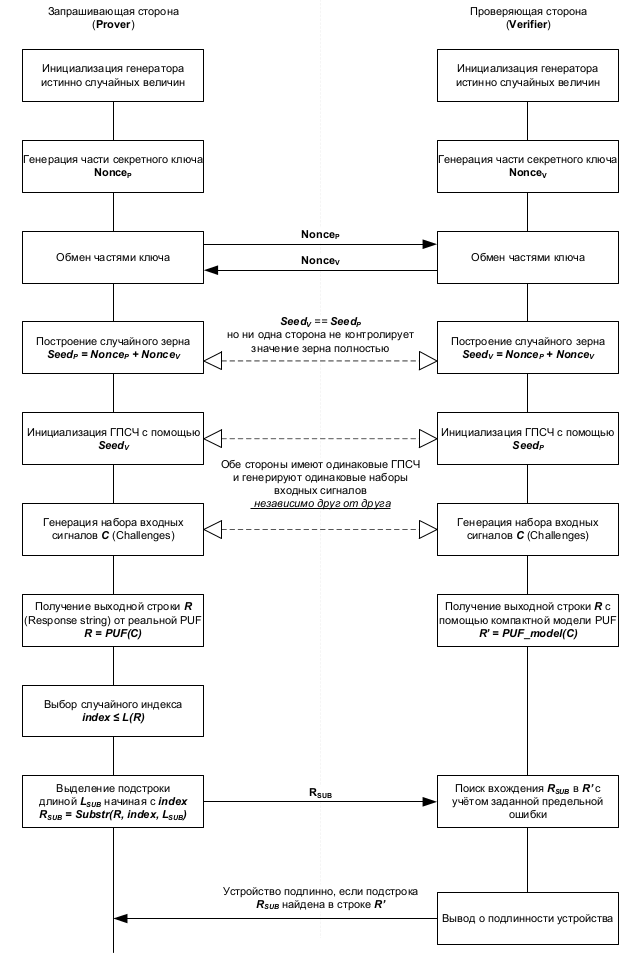
\includegraphics[width=0.93\textwidth]{protocol.png}
    \caption{Схема протокола аутентификации}
    \label{fig:architecture:protocol}
\end{figure}
% }

\clearpage
Набор функций, реализованных в библиотеке, напрямую определяется требованиями протокола. Библиотека предоставляет следующий функционал, используемый как клиентской, так и серверной частью:
\begin{itemize}
  \item Класс-обёртка TRNG для генерации истинно случайных значений с использованием системного генератора случайных чисел. Например в ОС Linux таковым является специальное устройство \emph{/dev/urandom}, предоставляющее интерфейс к пулу случайной информации, сгенерированной драйверами устройств путём сбора метрик шумовых процессов, протекающих при их работе. Применительно к протоколу TRNG используется для получения случайного зерна для PRNG и случайного индекса выходной подпоследовательности в режиме аутентификации и генерации запросов \emph{Challenge} для обучения модели в режиме регистрации.
  \item Класс-обёртка PRNG для генерации псевдослучайных значений. Использует реализацию алгоритма вихря Мерсенна из стандартной библиотеки языка Python. Требует инициализации с помощью зерна. PRNG используется для генерации запросов \emph{Challenge} в режиме аутентификации.
  \item Абстрактный класс Party для обозначения участников взаимодействия по протоколу. Предоставляет реализующим его классам функционал, общий для всех участников: методы идентификации в системе, методы обмена частями случайного зерна, методы генерации псевдослучайных последовательностей входных запросов.
  \item Класс Verifier, реализующий абстрактный класс Party. Представляет сущность сервера проверки подлинности и содержит методы для этапов протокола, специфичных для проверяющей стороны.
  \item Класс Prover, реализующий абстрактный класс Party. Представляет сущность клиентского приложения, представляющего устройство и содержит методы для этапов протокола, специфичных для стороны, запрашивающей проверку.
  \item Класс Configuration, представляющий собой набор конфигурационных параметров протокола и поддерживает инициализацию с помощью файла настроек или системных переменных окружения в дополнение к инициализации с помощью стандартных параметров конструктора.
\end{itemize}

Класс Configuration разобран чуть подробнее, так как от правильного его использования зависит применение параметров работы протокола, влияющих главным образом, на процент ложных срабатываний или наоборот, ложных отказов.
\clearpage
\lstinputlisting[
    style=commonstyle,
    firstline=5,
    caption={Класс Configuration},
    label=lst:architecture:configuration
]{src/configuration.py}

В таблице \ref{table:architecture:cfg_items} приведены краткие описания доступных параметров:

\begin{table}[ht]
  \caption{Параметры протокола аутентификации}
  \label{table:architecture:cfg_items}
  \begin{tabular}{| >{\raggedright}m{0.45\textwidth}
                  | >{\raggedright\arraybackslash}m{0.5\textwidth}|}
   \hline
   Параметр & Описание
   \\ \hline
   \textit{NONCE\_SIZE} & Длина (в битах) половины случайного зерна (результирующее зерно будет иметь длину \textit{2xNONCE\_SIZE}), используемого для инициализации ГПСЧ
   \\ \hline
   \textit{SUBSTR\_LEN} & Длина (в битах) извлекаемой из ответа реального устройства подстроки
   \\ \hline
   \textit{THRESHOLD} & Максимальное значение расстояния Хэмминга между строками, при котором они всё еще считаются схожими
   \\ \hline
   \textit{RSP\_LEN} & Фиксированная длина (в битах) ответа устройства (используется только для тестирования!)
   \\ \hline
  \end{tabular}
\end{table}

В следующих подразделах будут рассмотрены две стороны, взаимодействующие в рамках протокола.

\subsection{Модуль контроля доступа (клиентская часть)}
Так как протокол аутентификации по сути является набором правил, регулирующих обмен информацией нескольких сторон (в данном случае двух), логично описать правила поведения каждой из сторон по отдельности. В реализуемом протоколе участвуют \emph{клиент} -- сторона, имеющая доступ к устройству и <<представляющая его интересы>> в процессе аутентификации и \emph{сервер} -- сторона, обладающая подтверждение подлинности устройства.

В данной упрощённой реализации клиент также контролирует доступ к ресурсу, запрашиваемому устройством. Простейший пример -- электронный ключ в виде устройства с PUF запрашивает доступ к некоторому ресурсу, защищённому электронным замком. Электронный замок ничего не знает о подлинности устройства, в свою очередь устройство не может в одиночку доказать свою подлинность, т.к. по умолчанию не является доверенным. Здесь устройство пользуется <<услугой>> клиента (Prover), который является посредником между устройством, доказывающим свою подлинность, и доверенным сервером, обладающим релевантной информацией насчёт неё. Посредник также контролирует электронный замок, т.е. контролирует, какие устройства могут иметь к секретному ресурсу по результатам процесса аутентификации. Совмещение ролей посредника и барьера, конечно же, не является обязательным и сделано для упрощения архитектуры программного средства и эти роли могут быть без особых проблем разделены для более тонкого контроля над всей инфраструктурой.

По правилам протокола аутентификации клиентский модуль выполняет следующие функции:
\begin{itemize}
  \item генерировать истинно случайные и псевдослучайные данные для использования в алгоритмах протокола;
  \item взаимодействовать с устройством, посылая наборы входных сигналов и считывая результаты на выходе;
  \item создавать компактную модель уPUF на этапе регистрации;
  \item взаимодействовать с сервером, обмениваясь с ним секретной информацией -- с помощью библиотеки requests и грамотного использования защищенных соединений  и клиентских сессий.
\end{itemize}

С добавлением роли барьера примешиваются дополнительно функции надёжного хранения ссылки на секретный ресурс и предоставления устройству ссылки на секретный ресурс  в случае успешной аутентификации.

Как можно увидеть, модуль клиентской стороны использует множество ранее описанных классов и функций, не описывая своих классов или структур данных. Основной задачей клиентского модуля является реализация алгоритма проведения операций регистрации и атуентификации с использованием уже созданных инструментов. В таблице~\ref{table:architecture:client_funcs} описано, как реализованы эти инструменты, на основе которых построен алгоритм, являющийся главной логикой клиентского модуля.

\begin{table}[ht]
  \caption{Функции клиентского модуля и их реализации}
  \label{table:architecture:client_funcs}
  \begin{tabular}{| >{\raggedright}m{0.45\textwidth}
                  | >{\raggedright\arraybackslash}m{0.5\textwidth}|}
   \hline
   Функция & С помощью чего реализована
   \\ \hline
   Генерация истинно случайных чисел & Класс TRNG модуля протокола аутентификации
   \\ \hline
   Генерация псевдослучайных чисел & Класс PRNG модуля протокола аутентификации
   \\ \hline
   Обмен битовыми строками входных и выходных сигналов с утройствами & Класс Device и его производные классы в слое взаимодействия с устройствами
   \\ \hline
   Создание компактной модели PUF & Класс-обёртка над модулем построения модели (для обеспечения интероперабельности языков Python и Haskell)
   \\ \hline
   Контроль доступа у секретным ресурсам & Внутренние функции модуля или опциональный внешний интерфейс.
   \\ \hline
  \end{tabular}
\end{table}

\subsection{Модуль проверки подлинности (серверная часть)}
В описанном выше протоколе \emph{сервер} является сущностью, располагающей информацией о подлинности зарегистрированных устройств. Эта информация представлена в виде компактных моделей PUF, созданных на этапе их регистрации.

Функционал сервера во многом повторяет таковой у клиента, именно поэтому было принято решение вынести общие функции в абстрактный класс Prover. Сервер использует свою реализацию этого класса -- Verifier.

На основании вышесказанного, серверный модуль проверки подлинности выполняет следующие функции:
\begin{itemize}
  \item генерировать истинно случайные и псевдослучайные данные для использования в алгоритмах протокола;
  \item взаимодействовать с моделью устройства, посылая наборы входных сигналов и считывая результаты на выходе;
  \item иметь доступ к хранилищу моделей PUF;
  \item использовать алгоритм нечеткого поиска строки для сравнения данных, полученных от реального устройства с данными, полученными от компактной модели;
  \item работать в режиме сервера, т.е. принимать и обрабатывать входящие запросы, все время находясь в ожидании новых запросов;
\end{itemize}


\lstinputlisting[
    style=commonstyle,
    firstline=18,
    caption={Метод нечеткого поиска подстроки с заданным порогом},
    label=lst:architecture:fuzzysearch
]{src/fulllisting/puf.py}

\begin{table}[ht]
  \caption{Функции серверного модуля и их реализации}
  \label{table:architecture:client_funcs}
  \begin{tabular}{| >{\raggedright}m{0.45\textwidth}
                  | >{\raggedright\arraybackslash}m{0.5\textwidth}|}
   \hline
   Функция & С помощью чего реализована
   \\ \hline
   Работа в качестве HTTP-сервера по защищенному протоколу & Веб-фреймворка Flask и его поддержка безопасных соединений и клиентских сессий.
   \\ \hline
   Генерация истинно случайных чисел & Класс TRNG модуля протокола аутентификации
   \\ \hline
   Генерация псевдослучайных чисел & Класс PRNG модуля протокола аутентификации
   \\ \hline
   Обмен битовыми строками входных и выходных сигналов с моделью PUF & Класс Model
   \\ \hline
   Работа с хранищилем моделей PUF & Класс Database и его реализации для работы с файловой системой, Redis или MongoDB
   \\ \hline
   Нечеткий поиск подстроки & Класс Response модуля PUF и его реализации нечеткого поиска
   \\ \hline
  \end{tabular}
\end{table}


Сервер проверки подлинности должен иметь возможность обмена данными с моделью образом, похожим на способ взаимодействия с устройствами для модуля контроля доступа. Для данной цели создан класс Model, который предоставляет такой же интерфейс к модели PUF, какой предоставляет слой взаимодействия с устройствами для реальных PUF. Метод \emph{f} класса Model принимает масиив битов класса Challenge и возвращает бит ответа -- объект класса Response.

Для взаимодействия с хранилищем моделей модуль проверки подлинности предоставляет простой класс Database, по умолчанию реализующий хранение моделей в виде файлов на файловой системе. В то время как такой подход может быть полезен при тестировании приложения, для реального использования стоит также рассмотреть другие варианты:
\begin{itemize}
  \item NoSQL база данных. Так как модели PUF являются независимыми наборами векторов, использование классической реляционной базы данных в данном случае нерационально, ведь модели не имеют множества атрибутов, как не имеют и связей и отношений с другими сущностями в БД. В рамках этого варианта программное средство поддерживает работу с нереляционной СУБД MongoDB.
  \item Кэш (неперсистентное хранилище). В зависимости от требований информационной системы, в которой планируется использование данного ПС, является вероятным сценарий того, что модели PUF не должны храниться в базе слишком долго, или даже могут являться одноразовыми. В данном случае можно использовать систему хранения временных данных в памяти (memcached, Redis). Более того, так как в системе принято условие <<одно устройство -- одна модель>>, можно обойтись простейшим хранилищем типа <<ключ-значение>>(\emph{key-value store}). Для этого варианта реализован класс для работы с хранилищем Redis.
\end{itemize}
